\section{Schroeder}

Con l’obiettivo di ricreare, passo dopo passo, le unità descritte nell’articolo
\emph{Natural Sounding Artificial Reverberation}\footcite{ms:rev62}, le prime
implementazioni in \faust~sono relative ai due blocchi essenziali, \emph{Comb}
e \emph{All-Pass}, e alle interazioni tra loro.

\subsection{Comb}

Il codice di studio del filtro \emph{Comb} descritto in fig. \ref{fig:dfl}, con
i passi di correzione del dei tempi di integrazione per l'ottenimento della
risposta all'impulso indicata da Schroeder e riportata in fig. \ref{fig:dflir}.

\lstinputlisting{Code/dflc.dsp}

\todo{sarebbe opportuno indicare le motivazioni della correzione del filtro}

Il l'algoritmo utilizza le variabili $t$ (unità di tempo di ritardo espressa in
campioni) e $g$ (coefficiente di riscalamento del segnale in feedback).

\begin{figure}[htp]
\centering
\includegraphics[width=0.80\textwidth]{Code/dflc-svg/process.pdf}
\caption{\emph{Delay Feedback Loop} con correzioni per l'implementazione
         digitale \emph{samplerate}: il modulo \emph{delay} opera un ritardo
         $t-1$ quindi con $t=1$ il ritardo accumulato internamente al ciclo di
         \emph{feedback} è $0$, il campione di ritardo per $x$ è recuperato dopo
         il ciclo di \emph{feedback}.}
\label{fig:dflfaust}
\end{figure}

\subsection{All-Pass}

Il secondo algoritmo implementato permette di ottenere un filtro All-Pass
con risposta impulsiva in frequenza e ampiezza identiche a quelle descritte
dall'autore con figura \ref{fig:apf}

\lstinputlisting{Code/msapf.dsp}

Il comportamento \emph{All-Pass} è dato dalla somma del segnale ritardato
scalato di $(1-g^2)$ e il segnale diretto per $-g$, scalato con inversione di
polarità.

\begin{figure}[htp]
\centering
\includegraphics[width=0.80\textwidth]{Code/msapf-svg/process.pdf}
\caption{\emph{All-Pass}}
\label{fig:apfaust}
\end{figure}

\subsection{Sequenza di All-Pass}

I filtri \emph{Comb} e \emph{All-Pass} implementati sono gli elementi basilari
della riverberazione artificiale di \ms. Di seguito espongo le implementazioni
articolate, dei filtri sopra descritti, che l'autore espone.

\lstinputlisting{Code/msapfseq.dsp}

\begin{figure}[htp]
\centering
\includegraphics[width=0.80\textwidth]{Code/msapfseq-svg/process.pdf}
\caption{Sequenza di \emph{All-Pass}}
\label{fig:apfseq}
\end{figure}

\subsection{Annidamento e controllo}

\ms, immediatamente dopo la creazione degli elementi base, espone una serie di
risultati sperimentali ottenuti nella ricerca della simulazione di alcuni dei
comportamenti del riverbero acustico. Uno di questi è la possibilità di annidare
un \emph{All-Pass} dentro un \emph{All-Pass} in modo che i due filtri combinati
possano:
\begin{enumerate}
  \item bilanciare il rapporto tra segnale diretto e segnale riverberato
  \item l'introduzione di un ritardo tra i due segnali (diretto e riverberato)
  \item una dipendenza del tempo di riverberazione dalla frequenza
\end{enumerate}

\lstinputlisting{Code/msapfdwp.dsp}

\begin{figure}[htp]
\centering
\includegraphics[width=0.80\textwidth]{Code/msapfdwp-svg/process.pdf}
\caption{All-Pass contenente una unità comb contenente una unità all-pass}
\label{fig:apfdwp}
\end{figure}

\begin{figure}[htp]
\centering
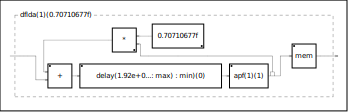
\includegraphics[width=0.80\textwidth]{Code/msapfdwp-svg/dflda-0x600001c847e0.pdf}
\caption{dfla: unità comb contenente un all-pass}
\label{fig:dfla}
\end{figure}

\subsection{Algoritmi Combinati}

Come già visto nel Capitolo 3, \todo{rifare puntatore al paragrafo corretto}
queste unità riverberanti, prese singolarmente, non risultano particolaremente
efficaci dal punto di vista della densità. Il passo successivo è quindi quello
di crare delle reti di riverberatori combinando queste unità fondamentali.

\lstinputlisting{Code/mscombapf.dsp}

\begin{figure}[htp]
\centering
\includegraphics[width=1\textwidth]{Code/mscombapf-svg/process.pdf}
\caption{Modello di riverberatore complesso di Schroeder: Filtri Comb in parallelo
         in filtri All-Pass in serie}
\label{fig:mscombapf}
\end{figure}

Quest'algoritmo risulta essere il più efficace ad ora e permette la
riproduzione di oltre $1000$ echi al secondo, un buon risultato considerando
le stime effettute da Schroeder, ma che non corrisponde ad una riverberazione
realistica e gradevole.

\lstinputlisting{Code/msapfcomb.dsp}

\todo[inline]{dovresti scrivere che il capovolgimento del flusso di elaborazione del
segnale non produce comportamenti differenti ed il riverbero calcolato è identico.
il sistema capovolto permette però la generazione di un segnale polifonico}

\begin{figure}[htp]
\centering
\includegraphics[width=1\textwidth]{Code/msapfcomb-svg/process.pdf}
\caption{Modello capovolto}
\label{fig:msapfcomb}
\end{figure}
